\documentclass[tikz, convert={outext=.png}]{standalone}

% use xelatex
\usepackage{fontspec}
\usepackage{pgffor}

\setmainfont{Ubuntu Mono}

\newcommand{\nullch}{\footnotesize{\textbackslash 0}}

\tikzstyle{arrgrid} = [rectangle, draw, minimum width = 0.5cm, minimum height = 0.5cm]

\begin{document}

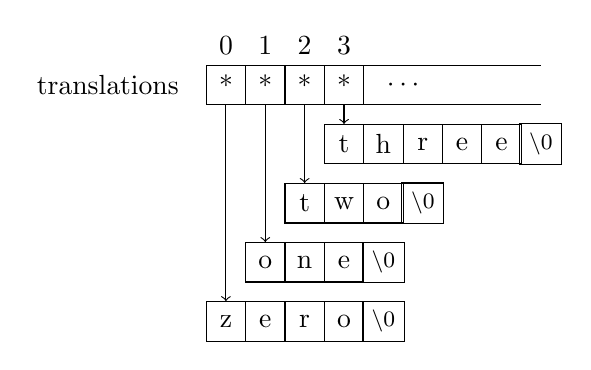
\begin{tikzpicture}
  \node at (-1.5, 0) {translations};
  \foreach \i in {0, 1, 2, 3} {
    \node[arrgrid] (r\i) at (\i * 0.5, 0) {*};
    \node at (\i  * 0.5, 0.5) {\i};
  }
  \draw[-] (1.75, 0.25) -- (4, 0.25);
  \draw[-] (1.75, -0.25) -- (4, -0.25);
  \node at (2.25, 0) {\(\cdots\)};
  \foreach \i\j in {0/z, 1/e, 2/r, 3/o, 4/\nullch} {
    \node[arrgrid] (zero\i) at (\i * 0.5, -3) {\j};
  }
  \foreach \i\j in {0/o, 1/n, 2/e, 3/\nullch} {
    \node[arrgrid] (one\i) at (\i * 0.5 + 0.5, -2.25) {\j};
  }
  \foreach \i\j in {0/t, 1/w, 2/o, 3/\nullch} {
    \node[arrgrid] (two\i) at (\i * 0.5 + 1, -1.5) {\j};
  }
  \foreach \i\j in {0/t, 1/h, 2/r, 3/e, 4/e, 5/\nullch} {
    \node[arrgrid] (three\i) at (\i * 0.5 + 1.5, -0.75) {\j};
  }
  \foreach \i\j in {0/zero, 1/one, 2/two, 3/three} {
    \draw[->] (r\i) -- (\j0);
  }
\end{tikzpicture}

\end{document}